\documentclass{sintefbeamer}

% packages, font, color, and newcommands
\usepackage{amsfonts, amsmath, oldgerm, lmodern, bm}
% \usepackage[font={footnotesize}]{caption}
\usepackage{natbib}
\usepackage{url}
\usepackage{tikz}
\usepackage{amssymb}
\usepackage{amsmath}
\usepackage{amsthm}
\usepackage{mathrsfs}
\usepackage{empheq}
\usepackage{mdframed}
\usepackage{bm}
\usepackage{animate}
\usepackage{xcolor,colortbl}
\usepackage{graphicx}
\usepackage{pgfplots}
\bibliographystyle{apalike}
\usefonttheme{serif}
\usetikzlibrary{calc}

% \title{Theoretical prediction of the Reynolds stress in low inertial buoyant emulsion.}
\title{Nearest particle statistics in rising monodisperse suspensions of drops.}
\subtitle{A theoretical study on pseudo turbulence}
\author{\href{https://scholar.google.com/citations?user=GQDBlaQAAAAJ&hl=en}{\underline{N. Fintzi}\footnote{IFP \'Energies Nouvelles, France}$^{,2}$}, JL. Pierson$^1$ and S. Popinet\footnote{Sorbonne Universit\'e, France}}
% \date{Created on May 22, 2022}

\titlebackground{image/800good.png}

% document body
\addtobeamertemplate{navigation symbols}{}{%
    \usebeamerfont{footline}%
    \usebeamercolor[fg]{footline}%
    % \hspace{1em}%
    % \vspace{1em}%
    \insertframenumber/\inserttotalframenumber
}
\usepackage{stmaryrd}

\usepackage{amsmath}


\begin{document}
\maketitle


\begin{frame}
  \frametitle{Industrial context}
  \underline{Buoyant emulsions are ubiquitous in chemical engineering processes :}
  \begin{itemize}
    \item Separation processes (gravity separators, flotation)
    \item Bubble column reactors
    \item Liquid-liquid separation
  \end{itemize}
  \vfill
  \pause
  \underline{In all those process we want to : }
  \begin{itemize}
    \item Predict global hydrodynamics using \textbf{Euler-Euler} averaged models. 
    \begin{itemize}
      \item Closure for the interphase drag forces, first moments of hydrodynamics forces, inter-particles forces.
      \item Closure of coalesce and break-up to predict the size distribution.
      \item Closure for the \textbf{Reynolds stress} or Pseudo-turbulent tensor :$\avg{\textbf{u}'\textbf{u}'}$.
      % \begin{itemize}
      %   \item Describe the interactions between pairs of droplets
      %   \item Predict interaction frequency
      %   \item Predict film drainage time 
      % \end{itemize}
    \end{itemize}
  \end{itemize}
\pause
  \vfill
$\to$ In this presentation we focus on the theoretical modeling of \textbf{Reynolds Stress}.
\end{frame}

\section{Introduction : what is the Reynolds stress ?}

\begin{frame}{To model the processes we use Euler-Euler framwork }
  Averaged \textbf{mass} and \textbf{momentum} equations for the continuous phase :
\begin{align*}
  % \phi_d + \phi_f &= 1\\
  \pddt (\phi_f \rho_f)  
  + \div (\phi_f \rho_f\textbf{u}_f)
  &= 
  0\\
  \pddt (\phi_f \rho_f\textbf{u}_f)  
  + \div (
      \phi_f \rho_f\textbf{u}_f\textbf{u}_f
      + \bm{\sigma}_f^\text{eff}
  )
  &= 
  \phi_f  \rho_f \textbf{g}
  + 
  \underbrace{
    \avg{\delta_I \bm{\sigma}_f^0 \cdot \textbf{n}_f}
  }_\text{Interphase force}
\end{align*}
With the effective stress : 
\begin{align*}
  &\bm{\sigma}_f^\text{eff}
  = 
   \underbrace{\rho_f\avg{\chi_f \textbf{u}_f'\textbf{u}_f'}}_\text{Reynolds stress}
    - \underbrace{\phi_f \bm{\sigma}_f}_\text{Newtonian stress}
\end{align*}
\begin{itemize}
  \item $\textbf{u}_f$ mean velocity of the continuous phase.  
  \item $\rho_f$ : density of the continuous phase. 
  \item $\phi_f$ : volume fraction of the continuous phase. 
  \item $\avg{\ldots}$ : the ensemble average operator. 
  \item $\textbf{u}_f' = \textbf{u}^0_f - \textbf{u}_f$ where $\textbf{u}_f^0$ is the local (non-averaged) fluid velocity. 
\end{itemize}
\end{frame}





\begin{frame}{Objectives and Hypothesis :}
  \begin{equation*}
     \avg{\chi_f \textbf{u}_f'\textbf{u}_f'}
     = 
     \text{Particle induced turbulence}
     + \text{Single phase turbulence}
  \end{equation*}
  \hrule\hrule
  \pause
  \begin{itemize}
    \item 
    Focus on the \textbf{Particle induced turbulence}. 
    \item Assuming : 
    \begin{itemize}
      \item Negligible inertia (\textbf{Stokes} regime)
      \item Dilute regime such that $\phi^{2} \approx 0$ 
      \item Mono-disperse suspension of droplets of radius $a$
    \end{itemize}
  \end{itemize}
\hrule\hrule
  \pause
  In this specific situation we can write  (Bachelor 1972) :
  \begin{equation*}
    \avg{\chi_f \textbf{u}'_f\textbf{u}'_f}(\textbf{x},t)
    = 
    n_p(\textbf{x},t)
    \int_{|\textbf{r}| > a }
     \textbf{u}^1\textbf{u}^1(\textbf{r}|\textbf{x}) d\textbf{r}
    +\mathcal{O}(\phi^2)
\end{equation*}

\begin{itemize}
  \item $\phi$ : dispersed phase volume fraction.
  \item $n_p = \frac{3\phi}{4\pi a^3}$ : number density of particles ;
  \item $\textbf{u}^1(\textbf{r}|\textbf{x})$ : disturbance field produce by a droplet located at \textbf{x}. 
\end{itemize}
\end{frame}

\begin{frame}
  \frametitle{L.Van Wijngaarden approach for potential flow.}

  \begin{columns}
    \column{0.8\textwidth}
Disturbance velocity field of an isolated translating bubble is :
\begin{equation*}
  \textbf{u}'_\text{pot}(\textbf{r})
  = \frac{a^3 \textbf{U}}{2}\left(\frac{\textbf{I}}{r^3} - \frac{3 \textbf{rr}}{r^5}\right)
  \text{    for    }r>a
\end{equation*}
\column{0.2\textwidth}
\includegraphics[width=\textwidth,angle=90]{image/Potential_cylinder.png}
\end{columns}
\pause
Therefore, the Reynolds stress approximation in homogeneous dilute suspension of spherical bubbles can be written Wijngaarden(1976): 
  \begin{align*}
    \avg{\chi_f \textbf{u}'_f\textbf{u}'_f}(\textbf{x},t)
    =
    n_p(\textbf{x},t)
      \int_{|\textbf{r}| > a }
       \textbf{u}_\text{pot}\textbf{u}_\text{pot}(\textbf{r}|\textbf{x}) d\textbf{r}
    = \phi \left(\frac{3}{20} U^2\textbf{I} + \frac{1}{20}\textbf{UU} \right)
\end{align*}

  \begin{itemize}
    \item $\phi$ is the volume fraction of the dispersed phase. 
    \item $\textbf{U} = \textbf{u}_f-\textbf{u}_p$ is the relative velocity between phases. 
    \item The integral converge because $\textbf{u}_\text{pot}  \sim r^{-3}$
  \end{itemize}
  \underline{$\to$ We aim for the same closure but in Stokes regime}
\end{frame}

\begin{frame}
  \frametitle{Stokes flow around a translating spherical drop}
  The stokes flow solution of an isolated translating drop is :
  \begin{columns}
    \column{0.6\textwidth}
  \begin{multline*}
    \textbf{u}_\text{stokes} 
    = \left(\frac{ \textbf{I}}{r} + \frac{\textbf{rr}}{r^3}\right)  \frac{1}{4}\left(\frac{3\lambda + 2}{\lambda +1}\right) a \textbf{U}\\
    - \left(-\frac{\textbf{I}}{r^3} + \frac{3 \textbf{rr} }{r^5}\right)  \frac{1}{4}\left(\frac{\lambda}{\lambda +1}\right) a^3 \textbf{U}
  \end{multline*}
  \begin{itemize}
      \item $\lambda$ is the viscosity ratio.
  \end{itemize}
  \column{0.3\textwidth}
  \begin{figure}
    % \caption{Disturbance velocity field of an isolated translating spherical droplet}
    \includegraphics[width=\textwidth]{image/Rising_Stokes.png}
  \end{figure}
  \end{columns}
\pause
  In this case : 
  \begin{align*}
    \avg{\chi_f \textbf{u}'_f\textbf{u}'_f}(\textbf{x},t) / n_p
    &\approx 
    \int_{|\textbf{r}| > a} \textbf{u}'_\text{stokes}\textbf{u}'_\text{stokes}   d\textbf{r}
    % - \phi_f \textbf{u}_f\textbf{u}_f
    =\infty 
  \end{align*}
  \underline{\textbf{The integral diverges}  ! (beacause $\textbf{u}_\text{stokes} \sim r^{-1}$).}



\end{frame}

\section{The Nearest Particle Statistics}
\transwipe[direction=90]
\begin{frame}{The Nearest Particle Statistics (NPS) approach (DZ Zhang, JFM, 2020)}
  $P_\text{nst}(\textbf{r}|\textbf{x})$ is the probability of finding a nearest particle at \textbf{r} knowing \textbf{x} is occupied by the continuous phase.   

  In the dilute, isotropic and homogeneous regime : 
  \begin{equation*}
    \boxed{P_\text{nst}(\textbf{r}|\textbf{x})
    = \frac{3\phi}{4\pi}
    e^{ - \phi (|\textbf{r}|^3 - 1) }
    \text{ for }
    |\textbf{r}| > a }
  \end{equation*}
  \pause
\begin{columns}
  \column{0.5\textwidth}
  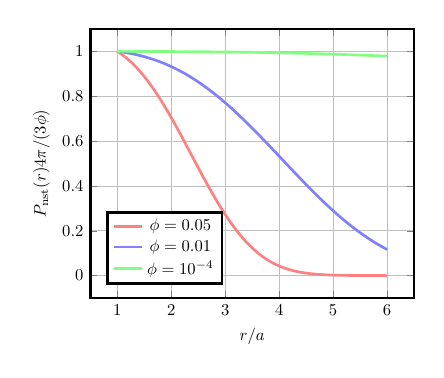
\begin{tikzpicture}[scale=0.6]
    \begin{axis}[
        xlabel={$r/a$},
        ylabel={$P_\text{nst}(r) 4\pi/ (3\phi) $},
        legend style={at={(0.05,0.05)}, anchor=south west},
        grid=major,
        domain=1:6,
        samples=100,
        ultra thick
    ]
    
    % Plot for phi = 0.05
    \addplot[color=red!50,ultra thick]
    { exp(-0.05 * (x^3 - 1))};
    \addlegendentry{$\phi = 0.05$}
    
    % Plot for phi = 0.01
    \addplot[color=blue!50,ultra thick]
    { exp(-0.01 * (x^3 - 1))};
    \addlegendentry{$\phi = 0.01$}
    
    % Plot for phi = 0.001
    \addplot[color=green!50,ultra thick]
    { exp(-0.0001 * (x^3 - 1))};
    \addlegendentry{$\phi = 10^{-4}$}
    
    \end{axis}
\end{tikzpicture}
\column{0.5\textwidth}
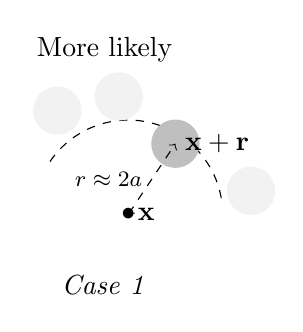
\begin{tikzpicture}[scale=0.6]
  \filldraw[ gray!10!white](+2.6,0.5)circle (0.5);
  \filldraw[ gray!10!white](-1.5,2.2)circle (0.5);
  \draw[dashed](10:2) arc (10:150:2);
  % \filldraw[ gray!50!white](0,0) circle (0.5);
  \filldraw[ gray!50!white](1,1.5)circle (0.5);
  \filldraw[ gray!10!white](-0.2,2.5)circle (0.5);
  \draw(0,0)node{$\bullet$}node[right]{$\textbf{x}$};
  \draw[dashed,<->](0,0)--(1,1.5)node[midway,left]{\footnotesize $r\approx 2 a$}node[right]{$\textbf{x}+\textbf{r}$};
  % \draw[dashed](-0.2,3.5);
  \node[ultra thick] (title) at (-0.5,3.5) {{More likely}};
  \node[ultra thick] (title) at (-0.5,-1.5) {\textit{Case 1}};
\end{tikzpicture} 
\hfill
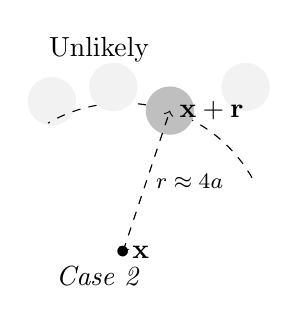
\begin{tikzpicture}[scale=0.6]
  \filldraw[ gray!10!white](+2.6,3.5)circle (0.5);
  \filldraw[ gray!10!white](-1.5,3.2)circle (0.5);
  \draw[dashed](30:3.16) arc (30:120:3.16);
  % \filldraw[ gray!50!white](0,0) circle (0.5);
  \filldraw[ gray!50!white](1,3)circle (0.5);
  \filldraw[ gray!10!white](-0.2,3.5)circle (0.5);
  \draw(0,0)node{$\bullet$}node[right]{$\textbf{x}$};
  \draw[dashed,<->](0,0)--(1,3)node[midway,right]{\footnotesize  $r\approx 4a$}node[right]{$\textbf{x}+\textbf{r}$};
  % \draw[dashed](-0.2,3.5);
  \node[ultra thick] (title) at (-0.5,4.3) {{Unlikely}};
  \node[ultra thick] (title) at (-0.5,-0.5) {\textit{Case 2}};
\end{tikzpicture} 


\end{columns}

\end{frame}


\begin{frame}
  \frametitle{The Reynolds stress decomposition with NPS}
  Using the relation between ensemble average $\avg{\ldots}$ and NPS average we obtain :
  \begin{equation*}
    \avg{\chi_f \textbf{u}'_f\textbf{u}'_f}(\textbf{x},t)
    = \phi_f
    \underbrace{\int 
      \textbf{u}^\text{nst}_f
      \textbf{u}^\text{nst}_f 
      P_\text{nst}(\textbf{r}|\textbf{x}) d\textbf{r} 
    }_\text{Averaged wake contribution}
    + \underbrace{ 
      \int \avg{\delta_i h_i \chi_f \textbf{v}_f''\textbf{v}_f''}  d\textbf{r}
    % P_{nst}(\textbf{x},t,\textbf{r}) d\textbf{r}
    }_{\mathcal{O}(\phi^2)}
  \end{equation*}

\begin{itemize}
  \item $\textbf{u}^\text{nst}(\textbf{x}|\textbf{y})$ disturbance velocity evaluated at \textbf{x}, knowing the nearest particle is located at $\textbf{y} = \textbf{x}+\textbf{r}$
  \item $\textbf{v}''_f = \textbf{u}^0_f - \textbf{u}^\text{nst}_f$ fluctuating values of the local velocity $\textbf{u}_f^0$ (non-averaged) around $\textbf{u}_f^\text{nst}$.
  \item This relation is exact and require no assumption. 
\end{itemize}
\end{frame}



\begin{frame}
  \frametitle{Stokes flow solution with NPS}
  \begin{small}
    \begin{equation*}
      \textbf{u}_\text{stokes} 
      = \left(\frac{ \textbf{I}}{r} + \frac{\textbf{rr}}{r^3}\right)  \frac{1}{4}\left(\frac{3\lambda + 2}{\lambda +1}\right) a \textbf{U}
      - \left(-\frac{\textbf{I}}{r^3} + \frac{3 \textbf{rr} }{r^5}\right)  \frac{1}{4}\left(\frac{\lambda}{\lambda +1}\right) a^3 \textbf{U}
    \end{equation*}
  \end{small}
  In the dilute regime we can write $\textbf{u}_f^\text{nst} = \textbf{u}_\text{stokes}$ thus,  :
  \begin{equation*}
    \avg{\chi_f \textbf{u}'_f\textbf{u}'_f}(\textbf{x},t)
    = 
    {\int \textbf{u}_\text{stokes} \textbf{u}_\text{stokes}  
    P_\text{nst}(r) d\textbf{r} }
    + \mathcal{O}(\phi^2)
  \end{equation*}\pause
  \footnotesize
  \begin{multline*}
    % - \phi_f \textbf{u}_f\textbf{u}_f\\
    =  
    + \left(\frac{9(2+3\lambda)^2 \Gamma(1/3)}{80 (\lambda +1)^2}\phi^{2/3} 
    - \frac{27+82\lambda + 62\lambda^2}{20(\lambda + 1)^2}\phi \right)\textbf{UU}
    + \left(\frac{(2+3\lambda)^2 \Gamma(1/3)}{240 (\lambda +1)^2}\phi^{2/3} 
     - \frac{1+6\lambda + 6\lambda^2}{20(\lambda + 1)^2}\phi \right)U^2\textbf{I} 
  \end{multline*}

  \begin{itemize}
    % \item  \textbf{Hypothesis 1} :$P_\text{nst}(\textbf{r}|\textbf{x}) = \frac{3\phi}{4\pi}
    % e^{ - \phi (r^3 - 1) }$
    % \item \textbf{Hypothesis 2} : We considered $\textbf{u}^\text{nst} = \textbf{u}_\text{stokes}$ since it is equivalent in the dilute regime
    \item Thanks to the fast decay of $P_\text{nst} \sim e^{-\phi (r^3-1)}$ the integral converges ! 
  \end{itemize}
  \begin{enumerate}
    \item $\Gamma(a) = \int_0^\infty t^{a-1} e^{-t} dt $ is the gamma  function. 
    \item  Notice that $\lim_{\phi \to 0} \avg{\chi_f \textbf{u}'_f\textbf{u}'_f}(\textbf{x},t)/\phi \sim\phi^{-1/3} =\infty$. 
    \item We found that $\avg{\chi_f \textbf{u}'_f\textbf{u}'_f}(\textbf{x},t)\sim\phi^{2/3}$ in agreement with Hill (2001) (ordered arrays solution). 
  \end{enumerate}
    
\end{frame}

\section{Comparison with DNS and experiment}

\section*{}
\begin{frame}
\frametitle{Direct Numerical Simulation of buoyant emulsions}
\begin{columns}
  \column{0.6\textwidth}
\underline{Simulation set up :} 
\begin{itemize}
  \item Tri -periodic boundary conditions. 
  \item Mono-disperse distribution of droplets size.
  \item We prevent coalesce by the use of a special algorithm 
  (\href{http://basilisk.fr/sandbox/fintzin/Rising-Suspension/no-coalescence.h}{no-coalescence.h})
  \item Free software : \url{https://basilisk.fr}
  \item Simulation source code : \url{http://basilisk.fr/sandbox/fintzin/Rising-suspension/RS.c}
\end{itemize}

\begin{figure}
  \caption{Snapshot of a simulation with $\phi = 0.01$, $Ga = 75$ $\lambda = 0.1$ and $N_b = 125$. In white : the interfaces, The background color map correspond to the pressure field. The grid represents the different core ($\approx 729$).
  }
\end{figure}
\column{0.5\textwidth}
\centering
\href{file:///work/fintzin/BUBLLES_PROJECT/movies/cut.gif}{\beamergotobutton{Play}}
\includegraphics[width =  1.1\textwidth]{image/PHI_01_Ga_75.png}
\end{columns}
\end{frame}

\begin{frame}
  \frametitle{Direct Numerical Simulation of buoyant emulsions}
  \begin{columns}
    \column{0.6\textwidth}
  \underline{Dimensionless parameters :} 
  \begin{itemize}
    \item \textit{Galileo} number : $Ga =\frac{\sqrt{\rho \Delta\rho g(2a)^3}}{\mu} \in [5, 100]$
    \item \textit{Bond} number : $Bo = \frac{\Delta \rho g (2a)^2}{\sigma} = 0.1$ 
    \item volume fraction of dispersed phase : $\phi = [0.01;0.2]$. 
    \item Density and viscosity ratio, $\rho_r=1.11$ and $\lambda= 0.1, 1, 10$. 
  \end{itemize}
  
  \begin{figure}
    \caption{Snapshot of a simulation for $\phi = 0.01$, $Ga = 75$ $\lambda = 0.1$ and $N_b = 125$. In white : the interfaces, The background color map correspond to the pressure field. The grid represents the different core ($\approx 729$).
    }
  \end{figure}
  \column{0.5\textwidth}
  \centering
  \includegraphics[width =  1.1\textwidth]{image/PHI_01_Ga_75.png}
  \end{columns}
\end{frame}


% \begin{frame}
%   \frametitle{Reconstruction of the velocity fields from DNS}
%   \begin{figure}[h!]
%     \centering
%     \begin{tikzpicture}
%         \node (img) at (0,0)  {\includegraphics[height=0.25\textwidth]{image/HOMOGENEOUS/Stream/Stream_PHI_5_Ga_10_l_1.pdf}};
%         \node (img) at (0.25\textwidth,0)  {\includegraphics[height=0.25\textwidth]{image/HOMOGENEOUS/Stream/Stream_PHI_5_Ga_100_l_1.pdf}};
%         \node (img) at (0.5\textwidth,0)  {\includegraphics[height=0.25\textwidth]{image/HOMOGENEOUS/Stream/Stream_PHI_5_Ga_10_l_10.pdf}};
%         \node (img) at (0.75\textwidth,0)  {\includegraphics[height=0.25\textwidth]{image/HOMOGENEOUS/Stream/Stream_PHI_5_Ga_100_l_10.pdf}};
%     \end{tikzpicture}
%     \caption{Nearest particle averaged velocity $\nstavg{\textbf{u}}(\textbf{r})$ for  $\phi = 5\%$ and $20\%$.
%     Green lines : contour plots of the nearest averaged indicator function $\nstavg{\chi_d}(\textbf{r})$ (it represent the mean shape of the particles)}
%     \label{fig:Stream}
%   \end{figure}
  
%   \begin{itemize}
%     \item Close from the drop ($r=\mathcal{O}(a)$) we can see that $\textbf{u}_\text{nst} \approx \textbf{u}_\text{stokes}$. 
%   \end{itemize}
% \end{frame}

% \begin{frame}
%   \frametitle{Nearest particle statistic solution for translating drops in stokes flow :}
%   \begin{multline}
%     \avg{\chi_f \textbf{u}'_f\textbf{u}'_f}(\textbf{x},t)
%     = 
%     {\int_a^\infty \textbf{u}_\text{stokes} \textbf{u}_\text{stokes}  P_{nst}(\textbf{x},t,\textbf{r}) d\textbf{r} }
%     - \phi_f \textbf{u}_f\textbf{u}_f
%     \\=
% -\left({{-\left(9\,\Gamma\left(-1 , \,\phi\right)\,\lambda^2\,\phi
% ^{{{4}\over{3}}}\,e^{\phi}\right)+\ldots}\over{\left(120\,\lambda^2+240\,\lambda+
% 120\right)\,\phi^{{{1}\over{3}}}}}\right)
% \textbf{e}_U\textbf{e}_U + \ldots
% \end{multline}
% \begin{itemize}
%   \item $\textbf{e}_U$ is the units vector in the direction of the drift velocity. 
% \end{itemize}

% \end{frame}

\begin{frame}
  \frametitle{Comparison with DNS results and experiments}
  \begin{figure}[h!]
    \centering    
    % \includegraphics[height = 0.25\textwidth]{image/upupexp.png}
    \includegraphics[height = 0.25\textwidth]{image/HOMOGENEOUS_NEW/CA/cartellier.pdf}
    \includegraphics[height = 0.25\textwidth]{image/HOMOGENEOUS_NEW/CA/UUyy.pdf}
    \caption{
       Dimensionless vertical component of the Reynolds stress :
       (left) Comparison with the rising bubbles experiment of Cartellier (2009) with $Re \approx 10$. 
       (right) comparison with DNS for two viscosity ratio $\lambda =1,10$ and $Re \approx 1$ DNS. 
    }
    \label{fig:Cp}
\end{figure}  
\begin{itemize}
  \item Good trends in terms of $\phi$ and $\lambda$.  
  \item Quantitative agreement for $\phi < 0.01$.  
\end{itemize}
\end{frame}


\begin{frame}
  {Going further}
  Toward a more complete model of \textbf{Bubble induced turbulence} : 
  \small
  \begin{multline*}
    \avg{\chi_f  \textbf{u}_f' \textbf{u}_f'}
    =
    \underbrace{
      C_1(\phi)\textbf{UU}
    + C_2(\phi)U^2 \textbf{I}
    + \overbrace{C_1(\phi)\avg{\textbf{u}_p'\textbf{u}_p'}
    + C_2(\phi)\avg{\textbf{u}_{p}'\cdot \textbf{u}_{p}'}\textbf{I}
    }^{\text{Particle center of mass velocity fluctuations}}
    }_\text{Particle Induced Turbulence (PIT)}
    % }_\text{Bubble induced turbulence in a uniform flow}
    % \\
  \end{multline*}
  \pause
  \begin{multline*}
    + \underbrace{\frac{\phi_d a^2 }{105 (\lambda +1)^2 }\left[
        (129\lambda^2+108\lambda+24)\textbf{E}_f\cdot \textbf{E}_f
        + (20\lambda^2 +20\lambda + 6)
        (\textbf{E}_f : \textbf{E}_f)\textbf{I}
    \right]}_\text{Shear Particle Induced Turbulence (S-PIT)}
\end{multline*}
\begin{columns}
  \column{0.5\textwidth}
  \begin{itemize}
    \item $\avg{\textbf{u}_p'\textbf{u}_p'}$ Particles center of mass velocity fluctuation.  
    \item $\textbf{E}_f$ Mean fluid phase shear rate. 
  \end{itemize}
  \begin{align*}
    C_{1} = \left(\frac{9(2+3\lambda)^2 \Gamma(1/3)}{80 (\lambda +1)^2}\phi^{2/3} 
    - \ldots\right)\\
    % C_2 = \left(\frac{9(2+3\lambda)^2 \Gamma(1/3)}{80 (\lambda +1)^2}\phi^{2/3} 
    % - \frac{27+82\lambda + 62\lambda^2}{20(\lambda + 1)^2}\phi \right)
  \end{align*}
  \column{0.2\textwidth}
  \begin{figure}
    \caption{Disturbance velocity field of a droplet immersed in a pure linear flow}
  \end{figure}
  \column{0.4\textwidth}
  \includegraphics[width=0.6\textwidth]{image/Shear_Stokes.png}
\end{columns}
\end{frame}

% \begin{frame}
%   \frametitle{perspectives}

%   \begin{itemize}
%     \item Compute the Ossen wake contribution to the Reynolds stress. 
%     \item Extend the model validity with DNS results. 
%   \end{itemize}

% \end{frame}

\backmatter

\begin{frame}
  \frametitle{Potential flow solution with NPS}
  In the dilute regime we can write 
  \begin{multline*}
    \avg{\chi_f \textbf{u}'_f\textbf{u}'_f}(\textbf{x},t)
    = 
    {\int \textbf{u}_\text{pot} \textbf{u}_\text{pot}  
    P_\text{nst}(r) d\textbf{r} }
    % - \phi_f \textbf{u}_f\textbf{u}_f\\
    =  \left(\frac{3}{20} U^2\textbf{I} + \frac{1}{20}\textbf{UU} \right)
    \underline{\Gamma_\text{inc}(-1,\phi)\phi^2 e^\phi}
  \end{multline*}

  \begin{itemize}
    \item  \textbf{Hypothesis 1} :$P_\text{nst}(\textbf{r}|\textbf{x}) = \frac{3\phi}{4\pi}
    e^{ - \phi (r^3 - 1) }$
    \item \textbf{Hypothesis 2} : We considered $\textbf{u}^\text{nst} = \textbf{u}_\text{potential}$ since it is equivalent in the dilute regime
    \item $\Gamma_\text{inc}(a,x) = \int_x^\infty t^{a-1} e^{-t} dt $ is the incomplete gamma  function. 
  \end{itemize}

  $\to$ Notice that $\Gamma_\text{inc}(-1,\phi)\phi^2 e^\phi \approx  \phi + \mathcal{O}(\phi^2)$ Therefore, we recover  Wijngaarden(1976) solution ! 

\end{frame}


\begin{frame}
  \frametitle{Comparison with DNS results and experiments}
  \begin{figure}[h!]
    \centering    
    % \includegraphics[height = 0.25\textwidth]{image/upupexp.png}
    \includegraphics[height = 0.25\textwidth]{image/HOMOGENEOUS_NEW/CA/UUyy.pdf}
    \includegraphics[height = 0.25\textwidth]{image/HOMOGENEOUS_NEW/CA/UUyykp.pdf}
    \caption{
       Dimensionless vertical component of the Reynolds stress :
       (left) Without the contribution from the particle phase velocity fluctuation . 
       (left) Including the contribution from the particle phase velocity fluctuation . 
    }
    \label{fig:Cp}
\end{figure}  
\begin{itemize}
  \item A slight improvement is observed
\end{itemize}
\end{frame}


\end{document}

